\section{Package ViewModel}
\begin{figure}[h!]
\begin{center}
	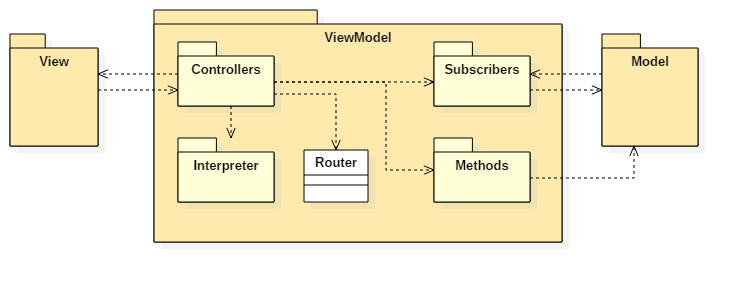
\includegraphics[scale=0.7]{../images/ViewModelPackage.png}
\end{center}
\end{figure}
\subsection{ViewModel::Controllers}
\subsubsection{ViewModel::Controllers::NewQuestionController}
\begin{itemize}
\item\textbf{Funzione del componente}: la classe permette di gestire la creazione di una nuova domanda
	\item\textbf{Relazione d'uso con altre componenti}: \\
La classe utilizza:
	\begin{itemize}
		\item ViewModel::Methods::QuestionMethods
		\item View::Templates::QuestionForm
	\end{itemize}
\item\textbf{Attributi}:
	\begin{itemize}
		\item\code{- \$scope}: Campo dati contenente un riferimento all’oggetto \$scope creato da Angular, viene utilizzato come mezzo di comunicazione tra il controller e il template.\\
	\end{itemize}
\item\textbf{Metodi}:
	\begin{itemize}
		\item\code{+ NewQuestionController()}: metodo costruttore della classe\\
		\textbf{Parametri}:
			\begin{itemize}
				\item\code{\$scope}: campo dati contenente un riferimento all’oggetto \$scope creato da Angular, viene utilizzato come mezzo di comunicazione tra il controller e il template.\\
			\end{itemize}
		\item\code{+ saveQuestion()}: metodo che permette il salvataggio di una nuova domanda tramite la chiamata ad un Method.\\
		\textbf{Parametri}:
			\begin{itemize}
				\item\code{question: String}: il testo QML della domanda da salvare.\\
				\item\code{category: String}: la categoria della domanda da salvare.\\
			\end{itemize}
	\end{itemize}
\end{itemize}

\subsubsection{ViewModel::Controllers::NewQuizController}
\begin{itemize}
\item\textbf{Funzione del componente}: la classe permette di gestire la creazione di un nuovo quiz (questionario);
\item\textbf{Relazioni con altre componenti}: \\
La classe utilizza:
	\begin{itemize}
		\item ViewModel::Methods::QuizMethods
		\item View::Templates::QuizCreationForm
	\end{itemize}
\item\textbf{Attributi}:
	\begin{itemize}
		\item\code{-\$scope}: Campo dati contenente un riferimento all'oggetto \$scope creato da Angular, viene utilizzato come mezzo di comunicazione tra il controller e il template.\\
	\end{itemize}
\item\textbf{Metodi}:
	\begin{itemize}
		\item\code{+ NewQuizController()}: metodo costruttore della classe\\
		\textbf{Parametri}:
			\begin{itemize}
				\item\code{\$scope}: campo dati contenente un riferimento all’oggetto \$scope creato da Angular, viene utilizzato come mezzo di comunicazione tra il controller e il template.\\
			\end{itemize}
		\item\code{+ saveQuiz()}: metodo per richiedere il salvataggio del nuovo quiz\\
		\textbf{Parametri}:
			\begin{itemize}
				\item\code{title: String}: il titolo del questionario.\\
				\item\code{categories: Array}: la lista delle categorie associate al questionario.\\
				\item\code{questions: Array}: la lista di id delle domande che compongono il questionario.\\
				\item\code{time: Int}: il tempo massimo in minuti per la compilazione del questionario.\\
			\end{itemize}
	\end{itemize}
\end{itemize}

\subsubsection{ViewModel::Controllers::QuizListController}
\begin{itemize}
\item\textbf{Funzione del componente}:  la classe permette il caricamento e la visualizzazione della lista di quiz disponibili nel sistema
	\item\textbf{Relazione d'uso con altre componenti}:
La classe utilizza:
	\begin{itemize}
		\item View::Templates::QuizList
	\end{itemize}
\item\textbf{Attributi}:
	\begin{itemize}
		\item\code{\$scope}: Campo dati contenente un riferimento all’oggetto \$scope creato da Angular, viene utilizzato come mezzo di comunicazione tra il controller e il template.\\
	\end{itemize}
\item\textbf{Metodi}:
	\begin{itemize}
		\item\code{+ QuizListController()}: metodo costruttore della classe\\
		\textbf{Parametri}:
			\begin{itemize}
				\item\code{\$scope}: campo dati contenente un riferimento all’oggetto \$scope creato da Angular, viene utilizzato come mezzo di comunicazione tra il controller e il template.\\
			\end{itemize}
		\item\code{+ quizzes()}: metodo che ritorna la lista dei quiz del sistema.\\		
		\item\code{+ orderBy()}: metodo che permette l'ordinamento della lista di quiz.\\
		\textbf{Parametri}:
			\begin{itemize}
				\item\code{orderBy: String}: il parametro in base al quale riordinare la lista di quiz.\\
			\end{itemize}
	\end{itemize}
\end{itemize}

\subsubsection{ViewModel::Controllers::QuizDetailsController}
\begin{itemize}
\item\textbf{Funzione del componente}: la classe permette di visualizzare le informazioni generali di un quiz, una volta selezionato dalla lista dei quiz;
	\item\textbf{Relazione d'uso con altre componenti}: \\
La classe utilizza:
	\begin{itemize}
		\item View::Templates::QuizList
	\end{itemize}
\item\textbf{Attributi}:
	\begin{itemize}
		\item\code{- \$scope}: Campo dati contenente un riferimento all'oggetto \$scope creato da Angular, viene utilizzato come mezzo di comunicazione tra il controller e il template.\\
	\end{itemize}
\item\textbf{Metodi}:
	\begin{itemize}
		\item\code{+ QuizDetailsController()}: metodo costruttore della classe\\
		\textbf{Parametri}:
			\begin{itemize}
				\item\code{\$scope}: campo dati contenente un riferimento all’oggetto \$scope creato da Angular, viene utilizzato come mezzo di comunicazione tra il controller e il template.\\
			\end{itemize}
		\item\code{+ quizDetails()}: metodo che permette la visualizzazione dei dettagli di un quiz.\\
		\textbf{Parametri}:
			\begin{itemize}
				\item\code{quizID: String}: identificativo univoco del quiz da visualizzare.\\
			\end{itemize}
	\end{itemize}
\end{itemize}

\subsubsection{ViewModel::Controllers::DeleteQuestionController}
\begin{itemize}
\item\textbf{Funzione del componente}: la classe fornisce le funzionalità necessarie alla cancellazione di una domanda precedentemente creata;
	\item\textbf{Relazione d'uso con altre componenti}: \\
La classe utilizza:
	\begin{itemize}
		\item ViewModel::Methods::QuestionMethods
		\item View::Templates::QuestionList
	\end{itemize}
\item\textbf{Attributi}:
	\begin{itemize}
		\item\code{- \$scope}: Campo dati contenente un riferimento all’oggetto \$scope creato da Angular, viene utilizzato come mezzo di comunicazione tra il controller e il template.\\

	\end{itemize}
\item\textbf{Metodi}:
	\begin{itemize}
		\item\code{+ DeleteQuestionController()}: metodo costruttore della classe\\
		\textbf{Parametri}:
			\begin{itemize}
				\item\code{\$scope}: campo dati contenente un riferimento all’oggetto \$scope creato da Angular, viene utilizzato come mezzo di comunicazione tra il controller e il template.\\
			\end{itemize}
		\item\code{+ deleteQuestion()}: metodo per richiedere l'eliminazione di una domanda\\
		\textbf{Parametri}:
			\begin{itemize}
				\item\code{question: String}: identificativo univoco della domanda da eliminare\\
			\end{itemize}
	\end{itemize}
\end{itemize}

\subsubsection{ViewModel::Controllers::DeleteQuizController}
\begin{itemize}
\item\textbf{Funzione del componente}: la classe fornisce le funzionalità necessarie alla cancellazione di un quiz precedentemente creato;
	\item\textbf{Relazione d'uso con altre componenti}: \\
La classe utilizza:
	\begin{itemize}
		\item ViewModel::Methods::QuizMethods
		\item View::Templates::QuizList
	\end{itemize}
\item\textbf{Attributi}:
	\begin{itemize}
		\item\code{- \$scope}: Campo dati contenente un riferimento all’oggetto \$scope creato da Angular, viene utilizzato come mezzo di comunicazione tra il controller e il template.\\
	\end{itemize}
\item\textbf{Metodi}:
	\begin{itemize}
		\item\code{+ DeleteQuizController()}: metodo costruttore della classe\\
		\textbf{Parametri}:
			\begin{itemize}
				\item\code{\$scope}: campo dati contenente un riferimento all’oggetto \$scope creato da Angular, viene utilizzato come mezzo di comunicazione tra il controller e il template.\\
			\end{itemize}
		\item\code{+ deleteQuiz()}:  metodo per richiedere l'eliminazione di un quiz\\
		\textbf{Parametri}:
			\begin{itemize}
				\item\code{quiz: String}: identificativo univoco del quiz da eliminare\\
			\end{itemize}
	\end{itemize}
\end{itemize}

\subsubsection{ViewModel::Controllers::QuizManagementController}
\begin{itemize}
\item\textbf{Funzione del componente}: la classe permette di gestire la somministrazione di un questionario;
	\item\textbf{Relazione d'uso con altre componenti}: \\
La classe utilizza:
	\begin{itemize}
		\item View::Templates::QuestionCompilation
	\end{itemize}
\item\textbf{Attributi}:
	\begin{itemize}
		\item\code{- \$scope}: Campo dati contenente un riferimento all’oggetto \$scope creato da Angular, viene utilizzato come mezzo di comunicazione tra il controller e il template.\\
	\end{itemize}
\item\textbf{Metodi}:
	\begin{itemize}
		\item\code{+QuizManagementController()}: metodo costruttore della classe\\
		\textbf{Parametri}:
			\begin{itemize}
				\item\code{\$scope}: campo dati contenente un riferimento all'oggetto \$scope creato da Angular, viene utilizzato come mezzo di comunicazione tra il controller e il template.\\
			\end{itemize}
		\item\code{+ nextQuestion()}: funzione che ritorna la domanda successiva nel questionario\\
		\textbf{Parametri}:
			\begin{itemize}
				\item\code{question: String}: identificativo univoco della domanda\\
			\end{itemize}
		\item\code{+ previousQuestion()}: funzione che ritorna la domanda precedente nel questionario\\
		\textbf{Parametri}:
			\begin{itemize}
				\item\code{question: String}: identificativo univoco della domanda\\
			\end{itemize}
		\item\code{+ endQuiz()}: metodo per la consegna del quiz in compilazione\\
	\end{itemize}
\end{itemize}

\subsubsection{ViewModel::Controllers::QuestionsManagementController}
\begin{itemize}
\item\textbf{Funzione del componente}: la classe permette di gestire la somministrazione di una singola domanda all'interno di un questionario;
	\item\textbf{Relazione d'uso con altre componenti}: \\
La classe utilizza:
	\begin{itemize}
		\item View::Templates::QuestionCompilation
		\item ViewModel::Methods::QuestionMethods
	\end{itemize}
\item\textbf{Attributi}:
	\begin{itemize}
		\item\code{- \$scope}: Campo dati contenente un riferimento all’oggetto \$scope creato da Angular, viene utilizzato come mezzo di comunicazione tra il controller e il template.\\
	\end{itemize}
\item\textbf{Metodi}:
	\begin{itemize}
		\item\code{+ QuestionsManagementController()}: metodo costruttore della classe\\
		\textbf{Parametri}:
			\begin{itemize}
				\item\code{\$scope}: campo dati contenente un riferimento all’oggetto \$scope creato da Angular, viene utilizzato come mezzo di comunicazione tra il controller e il template.\\
			\end{itemize}
		\item\code{+ getQuestion()}: metodo per caricare una domanda specifica\\
		\textbf{Parametri}:
			\begin{itemize}
				\item\code{question: String}: identificativo univoco della domanda\\
			\end{itemize}
	\end{itemize}
\end{itemize}

\subsubsection{ViewModel::Controllers::QMLEditorController}
\begin{itemize}
\item\textbf{Funzione del componente}: fornisce le funzionalità per creare e modificare una domanda tramite editor QML;
	\item\textbf{Relazione d'uso con altre componenti}: \\
La classe utilizza:
	\begin{itemize}
		\item ViewModel::Controllers::NewQuestionController
		\item ViewModel::Methods::QuestionMethods
	\end{itemize}
\item\textbf{Attributi}:
	\begin{itemize}
		\item\code{- \$scope}: Campo dati contenente un riferimento all’oggetto \$scope creato da Angular, viene utilizzato come mezzo di comunicazione tra il controller e il template.\\
	\end{itemize}
\item\textbf{Metodi}:
	\begin{itemize}
		\item\code{+ QMLEditorController()}: metodo costruttore della classe\\
		\textbf{Parametri}:
			\begin{itemize}
				\item\code{\$scope}: campo dati contenente un riferimento all’oggetto \$scope creato da Angular, viene utilizzato come mezzo di comunicazione tra il controller e il template.\\
			\end{itemize}
		\item\code{check()}: metodo che controlla che il testo QML inserito sia sintatticamente corretto\\
		\textbf{Parametri}:
			\begin{itemize}
				\item\code{text: String}: il testo QML inserito\\
			\end{itemize}
	\end{itemize}
\end{itemize}


\subsection{ViewModel::Subscribers}
\subsubsection{ViewModel::Subscribers::QuestionsSubscriber}
\begin{itemize}
\item\textbf{Funzione del componente}: la classe è necessaria ad effettuare il \emph{subscribe} relativo alla collezione di domande del sistema;
	\item\textbf{Relazione d'uso con altre componenti}: \\
La classe utilizza:
	\begin{itemize}
		\item Model::Publishers::QuestionsPublisher	
	\end{itemize}
\item\textbf{Attributi}:
	\begin{itemize}
		\item\code{- collection: String}: il nome della collezione sulla quale effettuare il subscribe.\\	
	\end{itemize}
\item\textbf{Metodi}:
	\begin{itemize}
		\item\code{+ getCollection(): String}: ritorna la collezione sulla quale può effettuare il subscribe.\\
		\item\code{+ subscribe()}: metodo che effettua il subscribe del parametro controller alla collezione\\
		\textbf{Parametri}:
			\begin{itemize}
				\item\code{controller: Object}: il controller che necessita della collezione\\
			\end{itemize}
	\end{itemize}
\end{itemize}

\subsubsection{ViewModel::Subscribers::QuizSubscriber}
\begin{itemize}
\item\textbf{Funzione del componente}: la classe è necessaria ad effettuare il \emph{subscribe} relativo alla collezione di quiz del sistema;
	\item\textbf{Relazione d'uso con altre componenti}:\\
La classe utilizza:
	\begin{itemize}
		\item Model::Publishers::QuizPublisher
	\end{itemize}
\item\textbf{Attributi}:
	\begin{itemize}
		\item\code{- collection: String}: il nome della collezione sulla quale effettuare il subscribe.\\	
	\end{itemize}
\item\textbf{Metodi}:
	\begin{itemize}
		\item\code{+ getCollection(): String}: ritorna la collezione sulla quale può effettuare il subscribe.\\
		\item\code{+ subscribe()}: metodo che effettua il subscribe del parametro controller alla collezione\\
		\textbf{Parametri}:
			\begin{itemize}
				\item\code{controller: Object}: il controller che necessita della collezione\\
			\end{itemize}
	\end{itemize}
\end{itemize}

\subsubsection{ViewModel::Subscribers::UsersSubscriber}
\begin{itemize}
\item\textbf{Funzione del componente}: la classe è necessaria ad effettuare il \emph{subscribe} relativo alla collezione di utenti del sistema;
	\item\textbf{Relazione d'uso con altre componenti}: \\
La classe utilizza:
	\begin{itemize}
		\item Model::Publishers::UserPublisher
	\end{itemize}
\item\textbf{Attributi}:
	\begin{itemize}
		\item\code{- collection: String}: il nome della collezione sulla quale effettuare il subscribe.\\
	\end{itemize}
\item\textbf{Metodi}:
	\begin{itemize}
		\item\code{+ getCollection(): String}: ritorna la collezione sulla quale può effettuare il subscribe.\\
		\item\code{+ subscribe()}: metodo che effettua il subscribe del parametro controller alla collezione\\
		\textbf{Parametri}:
			\begin{itemize}
				\item\code{controller: Object}: il controller che necessita della collezione\\
			\end{itemize}
	\end{itemize}
\end{itemize}

\subsection{ViewModel::Methods}
\subsubsection{ViewModel::Methods::QuestionMethods}
\begin{itemize}
\item\textbf{Funzione del componente}: permette al client di richiedere la modifica della collezione di domande del server;
	\item\textbf{Relazione d'uso con altre componenti}: \\
La classe utilizza:
	\begin{itemize}
		\item Model::Publishers::QuestionPublisher
	\end{itemize}
\item\textbf{Attributi}:
	\begin{itemize}
		\item\code{- collection: String}: la collezione sulla quale verranno implementati i methods\\
	\end{itemize}
\item\textbf{Metodi}:
	\begin{itemize}
		\item\code{+ insert()}: metodo che inserisce una domanda nella collezione\\
		\textbf{Parametri}:
			\begin{itemize}
				\item\code{questionId: String}: identificativo univoco della domanda da aggiungere\\
			\end{itemize}
		\item\code{+ remove()}: metodo che rimuove una domanda dalla collezione\\
		\textbf{Parametri}:
			\begin{itemize}
				\item\code{questionId: String}: identificativo univoco della domanda da rimuovere\\
			\end{itemize}
	\end{itemize}
\end{itemize}

\subsubsection{ViewModel::Methods::QuizMethods}
\begin{itemize}
\item\textbf{Funzione del componente}: permette al client di richiedere la modifica della collezione di quiz del server;
	\item\textbf{Relazione d'uso con altre componenti}: \\
La classe utilizza:
	\begin{itemize}
		\item Model::Publishers::QuizPublisher
	\end{itemize}
\item\textbf{Attributi}:
	\begin{itemize}
		\item\code{- collection: String}: la collezione sulla quale verranno implementati i methods\\
	\end{itemize}
\item\textbf{Metodi}:
	\begin{itemize}
		\item\code{+ insert()}: metodo che inserisce un quiz nella collezione\\
		\textbf{Parametri}:
			\begin{itemize}
				\item\code{quizId: String}: identificativo univoco del quiz da aggiungere\\
			\end{itemize}
		\item\code{+ remove()}: metodo che rimuove un quiz dalla collezione\\
		\textbf{Parametri}:
			\begin{itemize}
				\item\code{quizId: String}: identificativo univoco della domanda da rimuovere\\
			\end{itemize}
	\end{itemize}
\end{itemize}

\subsubsection{ViewModel::Methods::UserMethods}
\begin{itemize}
\item\textbf{Funzione del componente}: permette al client di richiedere la modifica della collezione di utenti del server;
	\item\textbf{Relazione d'uso con altre componenti}: \\
La classe utilizza:
	\begin{itemize}
		\item Model::Publishers::UserPublisher
	\end{itemize}
\item\textbf{Attributi}:
	\begin{itemize}
		\item\code{- collection: String}: la collezione sulla quale verranno implementati i methods\\
	\end{itemize}
\item\textbf{Metodi}:
	\begin{itemize}
		\item\code{+ insert()}: metodo che inserisce un utente nella collezione\\
		\textbf{Parametri}:
			\begin{itemize}
				\item\code{userId: String}: identificativo univoco dell'utente da aggiungere\\
			\end{itemize}
		\item\code{+ remove()}: metodo che rimuove un utente dalla collezione\\
		\textbf{Parametri}:
			\begin{itemize}
				\item\code{userId: String}: identificativo univoco dell'utente da rimuovere\\
			\end{itemize}
	\end{itemize}
\end{itemize}

\subsection{ViewModel::Interpreter}
\subsubsection{ViewModel::Interpreter::Interpreter}
\begin{itemize}
\item\textbf{Funzione del componente}: interfaccia di base del tipo Interpreter.
	\item\textbf{Relazione d'uso con altre componenti}: viene concretizzata in ViewModel::Interpreter::QMLInterpreter.\\ \\

\item\textbf{Attributi}: nessuno
\item\textbf{Metodi}:
	\begin{itemize}
		\item\code{+ translate(): String}: metodo astratto per la traduzione di un testo\\
		\textbf{Parametri}:
			\begin{itemize}
				\item\code{data: String}: l'input testuale che deve essere tradotto \\
			\end{itemize}
	\end{itemize}
\end{itemize}

\subsubsection{ViewModel::Interpreter::InterpreterFactory}
\begin{itemize}
\item\textbf{Funzione del componente}: interfaccia di base delle Factory di tipi Interpreter.
	\item\textbf{Relazione d'uso con altre componenti}: viene concretizzata da ViewModel::Interpreter::QMLInterpreterFactory.\\ 
\item\textbf{Attributi}: nessuno
\item\textbf{Metodi}:
	\begin{itemize}
		\item\code{+ createInterpreter(): Interpreter}: metodo astratto per la creazione di un Interpreter.\\
	\end{itemize}
\end{itemize}

\subsubsection{ViewModel::Interpreter::QMLInterpreterFactory}
\begin{itemize}
\item\textbf{Funzione del componente}: crea oggetti di tipo QMLInterpreter.
	\item\textbf{Relazione d'uso con altre componenti}: è concretizzazione dalla classe ViewModel::Interpreter::InterpreterFactory. Crea oggetti QMLInterpreter.\\
\item\textbf{Attributi}:
	\begin{itemize}
		\item\code{- instance: QMLInterpreterFactory}: campo dati statico che rappresenta l'unica istanza della classe\\
	\end{itemize}
\item\textbf{Metodi}:
	\begin{itemize}
		\item\code{- QMLInterpreterFactory()}: costruttore privato della classe\\
		\item\code{+ getInstance(): : QMLInterpreterFactory}: metodo che ritorna l'unica istanza della classe\\
		\item\code{+ createInterpreter(): QMLInterpreter}: metodo ereditato da InterpreterFactorye concretizzato per la creazione di un interprete di tipo QMLInterpreter.\\
	\end{itemize}
\end{itemize}

\subsubsection{ViewModel::Interpreter::QMLInterpreter}
\begin{itemize}
\item\textbf{Funzione del componente}: classe astratta che rappresenta gli Interpreter che traducono codice QML in un altro formato.
	\item\textbf{Relazione d'uso con altre componenti}: è sottotipo di ViewModel::Interpreter::Interpreter. Viene concretizzata in ViewModel::Interpreter::QML2HTMLInterpreter.\\ 
\item\textbf{Attributi}: Nessuno
\item\textbf{Metodi}:
	\begin{itemize}
		\item\code{translate(): String}: metodo astratto ereditato da Interpreter\\
		\textbf{Parametri}:
			\begin{itemize}
				\item\code{data: String}: l'input QML che deve essere tradotto \\
			\end{itemize}
	\end{itemize}
\end{itemize}

\subsubsection{ViewModel::Interpreter::QML2HTMLInterpreterFactory}
\begin{itemize}
\item\textbf{Funzione del componente}: traduce codice QML in codice HTML.
	\item\textbf{Relazione d'uso con altre componenti}: la classe è concretizzazione di ViewModel::Interpreter::QMLInterpreter.\\
\item\textbf{Attributi}: Nessuno
\item\textbf{Metodi}:
	\begin{itemize}
		\item\code{translate(): String}: metodo ereditato da QMLInterpreter e concretizzato per la traduzione di testo QML in testo HTML.\\
		\textbf{Parametri}:
			\begin{itemize}
				\item\code{data: String}: l'input QML che deve essere tradotto \\
			\end{itemize}
	\end{itemize}
\end{itemize}

\subsection{ViewModel::Router}
\subsubsection{ViewModel::Router::Router}
\begin{itemize}
\item\textbf{Funzione del componente}: implementa il routing dinamico dell'applicazione. Permette di dividere la parte statica dell'applicazione dalla parte che va caricata dinamicamente;
	\item\textbf{Relazione d'uso con altre componenti}: \\
La classe utilizza:
	\begin{itemize}
		\item ui-router
	\end{itemize}
\item\textbf{Attributi}:
	\begin{itemize}
		\item\code{\$locationProvider: \$locationProvider}: provider AngularJs per rendere gli Url più leggibili\\
		\item\code{\$urlRouterProvider: \$urlRouterProvider}: modulo del package ui-router per definire il routing di default dell'applicazione\\
		\item\code{\$stateProvider: \$stateProvider}: modulo del package ui-router per mappare gli Url al caricamento dinamico dei template dell'applicazione. Tale associazione è definita come uno 'state'\\
	\end{itemize}
\item\textbf{Metodi}:
	\begin{itemize}
		\item\code{state()}: metodo per collegare un Url dell'applicazione al rispettivo template da caricare\\
		\textbf{Parametri}:
			\begin{itemize}
				\item\code{state: String}: il nome dello stato rappresentato dall'associazione Url-Template\\
				\item\code{url: String}: l'Url sul quale effettuare il matching\\
				\item\code{template: String}: il template da caricare una volta trovato il match\\
			\end{itemize}
	\end{itemize}
\end{itemize}